\documentclass[conference]{IEEEtran}

% 4 oder 8 Seiten

\IEEEoverridecommandlockouts

\usepackage{cite}
\usepackage[pdftex]{graphicx}

\ifCLASSOPTIONcompsoc
  \usepackage[caption=false,font=normalsize,labelfont=sf,textfont=sf]{subfig}
\else
  \usepackage[caption=false,font=footnotesize]{subfig}

\usepackage[bookmarks=false]{hyperref}

\hyphenation{}

\newcommand{\citep}{\cite}

\begin{document}

\title{Performance Vergleich von Typ 1 und Typ 2 Hypervisoren }

\author
{
\IEEEauthorblockN{
	Colin Jochum, Tom Kleinhapl}
\IEEEauthorblockA{
	FH JOANNEUM -- University of Applied Sciences\\
	Dep. of Applied Computer Sciences\\
	Alte Poststra\ss e 147\\
	8020 Graz, Austria\\
	Supervisor: FH-Prof. Mag. Dr. Robert Singer}
}

\maketitle

\begin{abstract}
Diese Arbeit dreht sich um den Vergleich von Typ 1 und Typ 2 Hypervisoren hinsichtlich deren Performance. Die Forschungsfrage dieser Arbeit lautet, ob es einen signifikanten Unterschied ($>$10\%) hinsichtlich der CPU-Rechenleistung und der Boot Zeit zwischen den zwei Hypervisor Typen (Typ1, Typ2) gibt.
Um die Fragestellung zu beantworten, wurden zwei Messzenarien konzipiert. Der erste Messaufbau behandelt die Frage hinsichtlich der CPU-Rechenleistung. Hierbei kommt das CPU Benchmarking Tool Geekbench 5 zum Einsatz mit welchem sich sehr einfach die CPU Performance über ein Punktesystem vergleichen lässt. In diesem Test wurde sowohl die Single-Core sowie die Multi-Core Performance beider Hypervisoren verglichen. Zusätzlich wurden die Hypervisoren mit der Performance des Host Betriebssystems verglichen, um einen noch besseren Eindruck hinsichtlich der verringerten Leistung von Hypervisoren zu bekommen. Um zufällige Messfehler auszugleichen, wurden alle Geekbench Tests fünf Mal durchgeführt und der durchschnittliche Wert für die Interpretation des Ergebnisses herangezogen.
Der zweite Messaufbau beschäftigte sich mit dem Vergleich der Boot Zeit der beiden Hypervisor Typen. Hierzu wurde eine Kamera aufgestellt, welche die Zeit vom Start (Betätigen des Power On Buttons) bis zum Login Bildschirm filmt.
Die Ergebnisse des ersten Messzenarios brachten hervor, dass tatsächlich kein signifikanter Unterschied ($>$10\%) hinsichtlich der CPU-Rechenleistung zwischen den Hypervisoren besteht. Sowohl im Single-Core als auch im Multi-Core Benchmark erreichte der Hypervisor Typ 1 eine minimal bessere Leistung. Im Single-Core Benchmark betrug der Unterschied lediglich 3,40\% und im Multi-Core Benchmark betrug der Unterschied 5,33\%. Die Performance im Vergleich zum Host Betriebssystems war jedoch wie zu erwarten signifikant und Betrug bis zu 16\% im Single-Core Benchmark.
Das zweite Messzenario welches sich der Boot-Zeit annahm brachte hervor, dass der Typ 2 Hypervisor durchschnittlich 70\% länger brauchte als der Typ 1 Hypervisor. Hier ist ein signifikanter Unterschied von $>$10\% gegeben und lässt sich darauf zurückzuführen, dass beim Start eines Typ 2 Hypervisors wesentlich mehr Overhead involviert ist.

\end{abstract}

\IEEEpeerreviewmaketitle

\section{Einleitung}
\label{Einleitung}

Das Ziel dieser Arbeit ist es Performance Unterschiede zwischen Typ 1 und Typ 2 Hypervisoren zu untersuchen, um signifikante Abweichungen ($>$10\%) hinsichtlich CPU-Rechenleistung und Boot Zeit festzustellen. Dafür wurden zwei Mess-Szenarien entworfen und in einer Testumgebung durchgeführt. Im Kapitel der Arbeit werden theoretische Inhalte der Virtualisierung und der Nutzung von Hypervisoren erläutert, anschließend werden die Messungen und deren Ergebnisse dargelegt und interpretiert. Im letzten Kapitel werden mögliche Schlüsse aus den gewonnenen Erkenntnissen gezogen. 

\section{Virtualisierung und Hypervisoren}
\label{Virtualisierung und Hypervisoren}	
In der Informatik wird der Begriff der Virtualisierung primär mit der Virtualisierung von Hardwareressourcen assoziiert. Darunter versteht man die Nachbildung einer reellen Hardwareressource in einem standardisierten virtuellen Abbild mit Hilfe eines Abstraktions-Layers. Diese abstrahierende Schicht, die zwischen Hardware und Applikation, wird als Hypervisor, oder ursprünglich auch Virtual-Machine-Monitor (VMM) bezeichnet. [1] Durch die Abstraktion der zugrunde liegenden Ressourcen in logische, bietet ein Hypervisor eine virtuelle Umgebung für Betriebssysteme. Grundsätzlich müssen Hypervisoren drei wesentliche Aufgaben erfüllen: 
\begin{itemize}
	\item Eine Umgebung schaffen, die mit der physischen Umgebung ident ist. 
	\item Eine Umgebung mit minimalen Rechenleistungskosten bereitstellen. 
	\item Die Kontrolle über die Systemressourcen bewahren. 
\end{itemize}
[4]

Die ursprüngliche Bezeichnung von Hypervisoren als VMM stammt von deren primären Verwendungszweck der kompletten Systemvirtualisierung von Computern, nämlich das Ausführen von komplett voneinander isolierten Gasbeitriebsystemen in virtuellen Maschinen (VM). Die Form der Komplett-Virtualisierung steht auch im Fokus unserer Mess-Szenarien. Im Kontrast dazu gibt es auch die Paravirtualisierung, bei welcher sich mehrere Gasbetriebsysteme einen Kernel teilen. [2] Die Komplettvirtualisierung ermöglicht ebenfalls das Hosten mehrerer Betriebssysteme, allerdings benutzt hier jede Maschine einen eigenen Kernel. Der Hypervisor selbst erfüllt bei der Ressourcenallokation eine ähnliche Rolle wie ein Betriebssystem. Nur kommen Ressourcenanfragen nicht von einzelnen Anwendungen, sondern von einer VM. [1]

\subsection{Typ1 und Typ2 Hypervisoren}
Bei Hypervisoren wird generell zwischen zwei Architekturen unterschieden: Typ-1-Hypervisoren (auch native oder bare-metal Hypervisor) und Typ-2-Hypervisoren (auch hosted Hypervisor). Ein Typ-1 Hypervisor wird auch als nativer oder bare-metal Hypervisor beschrieben, weil dieser direkt auf der Server Hardware läuft, ohne ein darunterliegendes Betriebssystem zu benötigen. Ein typischer Typ-1 Hypervisor ist VMWare ESXi. Der Typ-2 Hypervisor oder auch hosted Hypervisor läuft über einem traditionellen Betriebssystem, dieses wird auch als Host-Betriebssystem bezeichnet. Ein typischer Typ-2 Hypervisor ist VMWare Workstation. Die verschiedenen Architekturen der beiden Hypervisor Typen werden in der Grafik 1 dargestellt. [2], [3] 

\begin{figure}[!h]
	\centering
	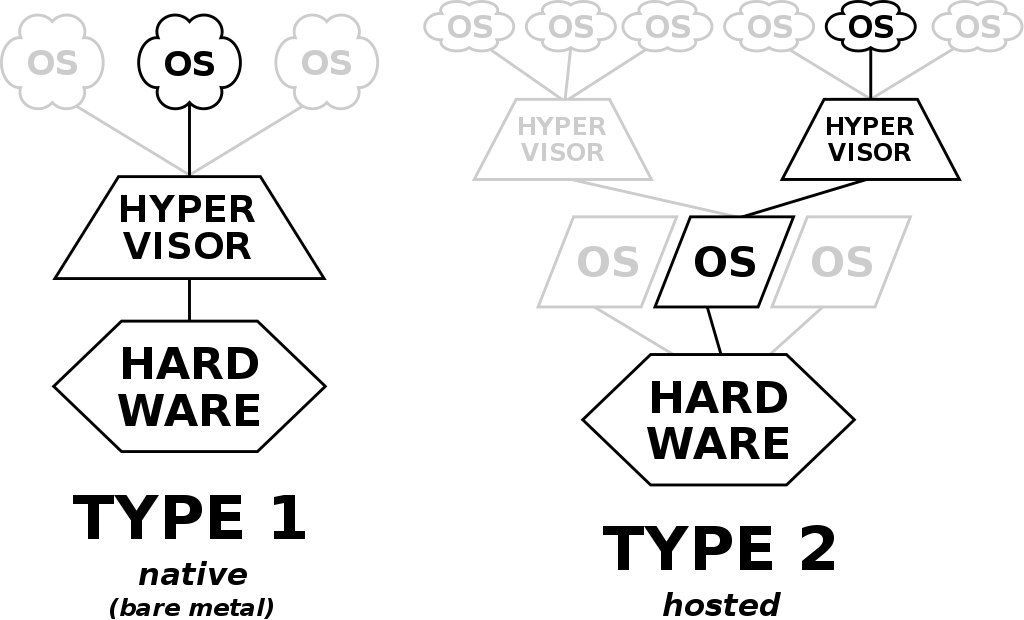
\includegraphics[keepaspectratio,width=8.5cm,height=0.75\textheight]{hypervisors.png}
	\caption{Die Architektur von Typ 1 und Typ 2 Hypervisoren.}
	\label{architecture}
\end{figure}

\section{Computer Spezifikation}
\label{Computer Spezifikation}
Die zwei Computersysteme welche für die Versuche/Messungen verwendet wurden, wurden von der FH Joanneum Graz zur Verfügung gestellt. Es wurden deshalb zwei Systeme ausgewählt da dadurch ein paralleler Testbetrieb ermöglicht wurde was eine enorme Zeitersparnis einbrachte. Bei den Systemen handelt sich um zwei vollständig idente Systeme um zu gewährleisten, dass die Grundvoraussetzungen dieselben sind. Die untenstehende Tabelle gibt einen Überblick über die wichtigsten Spezifikationen der beiden Systeme.

\begin{table}[!h]
\begin{tabular}{|l|l|}
\hline
CPU              & Intel Core i7-6700 4 Kerne + 4 Threads (3,40GHz) \\ \hline
SSD              & Samsung 500GB 860 EVO SSD                        \\ \hline
RAM              & 16GB DDR4 RAM                                    \\ \hline
Hypervisor Typ 1 & VMWare VSphere Hypervisor                        \\ \hline
Hypervisor Typ 2 & VMWare Workstation 16 Pro (30 Tage Testversion)  \\ \hline
OS               & Windows 10                                       \\ \hline
\end{tabular}
\end{table}

\section{Messung der CPU Performance}
\label{Messung der CPU Performance}
In diesem Kapitel wird die Leistung der CPU zwischen Hypervisor Typ 1 und Hypervisor Typ 2 verglichen. Es wird sowohl die Single Core Performance als auch die Multicore Performance gemessen.

\subsection{Messaufbau}
Für die Messung der CPU Performance haben wir uns dazu entschieden das Tool Geekbench in der derzeit aktuellen Version 5 zu verwenden. Bei Geekbench werden eine Vielzahl von unterschiedlichen Workloads durchgeführt um die Single-Core sowie die Multi-Core Performance zu testen [5]. Am Ende eines Testdurchlaufs berechnet Geekbench einen Score, welcher sich in unserem Aufbau sehr gut dazu eignet, die Hypervisortypen zu vergleichen. Die Spezifikationen des Testsystems lassen sich aus Kapitel 3 entnehmen.
Bei den Messungen haben wir sowohl die Single Core Performance als auch die Multicore Performance gemessen.  Die Messungen wurden 5-mal auf den zwei Virtualisierungsmethoden (Hypervisor Typ1, Hypervisor Typ2) durchgeführt, um Messfehler bzw. ungewollte Ausreiser durch eine Bildung des Mittelwerts auszugleichen.


\subsection{Single-Core Performance-Messung}
Bei der Single Core Performance Messung wird lediglich die Performance eines einzigen Rechenkerns gemessen. Dies bedeutet das Geekbench für den Benchmark eine vordefinierte CPU reserviert, um darauf den Benchmark durchzuführen. Vor der Durchführung des Experiments wurden theoretische Annahmen bezüglich der Unterschiede in den Scores zwischen Hypervisor Typ1 (esxi) und Typ2 (Vmware Workstation Pro) besprochen. Es ist zu erwarten, dass sich die Punkteanzahl bei einem Single Core Performance Benchmark zwischen den Hypervisoren nur marginal unterschiedet.
Wie bereits in Kapitel 3 erwähnt wurde der Single Core Benchmark insgesamt fünf Mal durchgeführt, um zufällig auftretende Messfehler später einfach mittels einer Mittelung auszugleichen. Die Resultate des Single Core Performance Tests mittels Geekbench 5 finden sich in der unterstehenden Grafik. \newline 

\begin{figure}[!h]
	\centering
	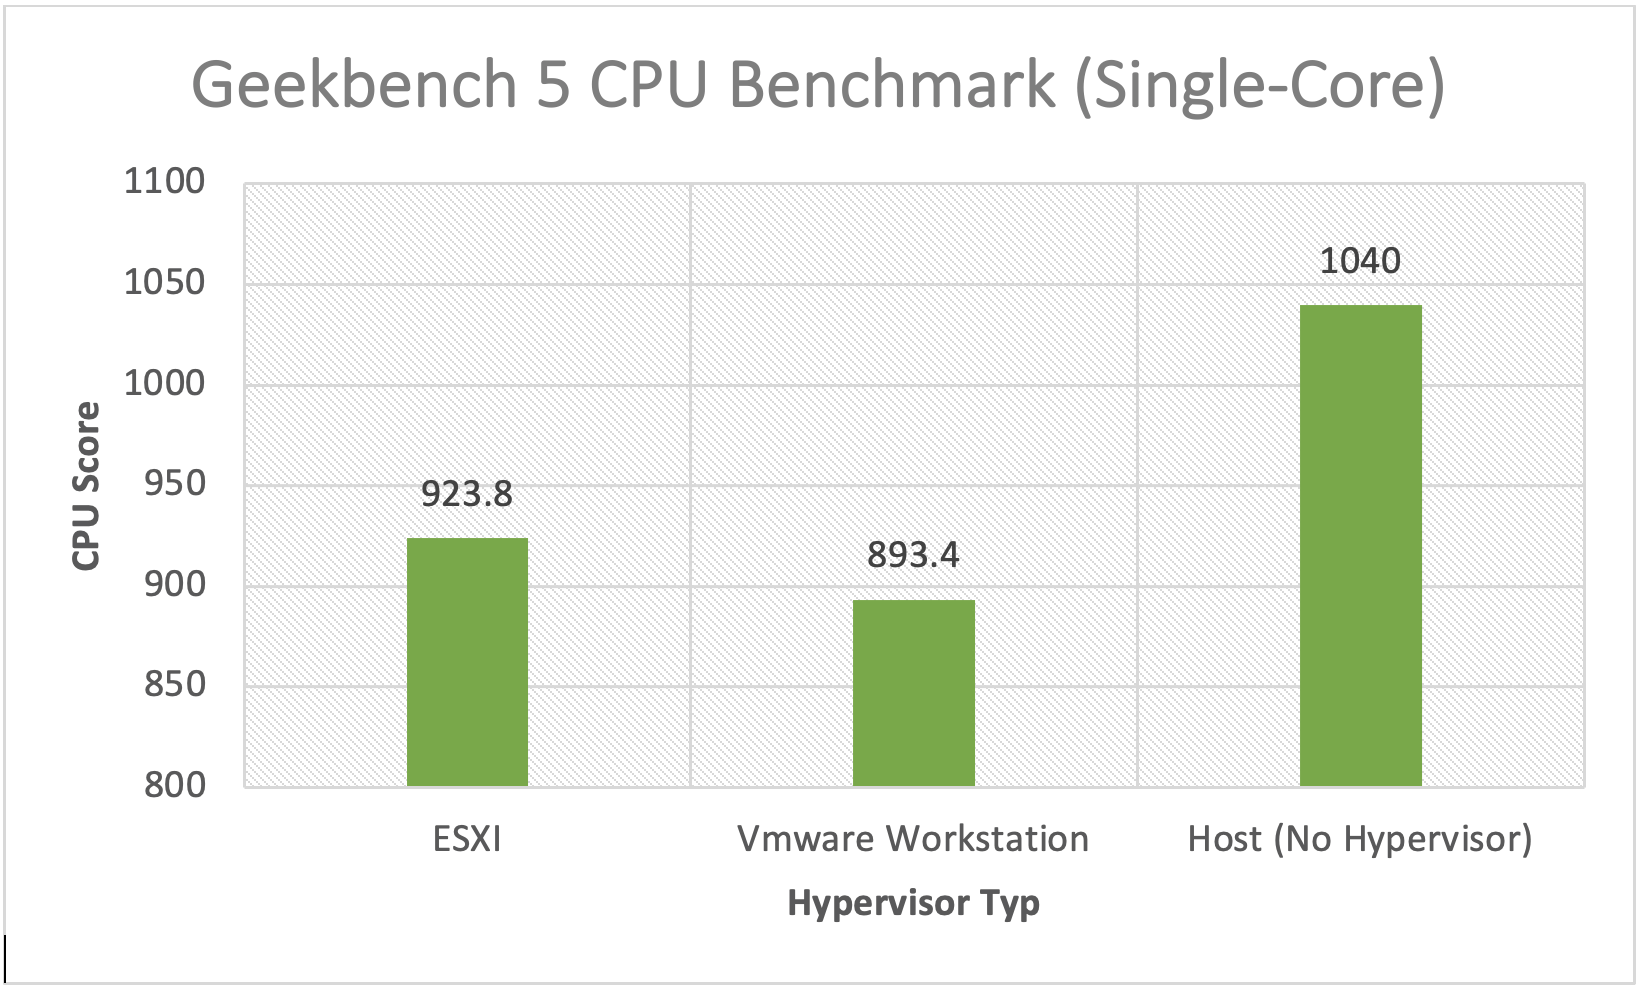
\includegraphics[keepaspectratio,width=8.5cm,height=0.75\textheight]{singlecore.png}
	\caption{Single Core Benchmark}
	\label{architecture}
\end{figure}

Wie angenommen unterschieden sich die Endergebnisse zwischen ESXI und VMWare Workstation Hypversior nur marginal. Der Typ 1 (ESXI) Hypervisor weißt wie zu erwarten eine höhere CPU Performance auf jedoch ist der Unterschied mit 30,4 Punkten (3,40\%) beinahe vernachlässigbar. Wesentlich höher fällt der Unterschied aus, wenn man das Single Core Punkteergebnis des Hosts (Kein Einsatz eines Hypervisors) mit den Hypervisor Resultaten vergleicht. Der Host erreichte im Single Core Performance Benchmark einen Wert von 1040 Punkten was im Vergleich zum ESXI Hypervisor ein Plus von 116,2 Punkten (12,57\%) bedeutet. Noch deutlicher fällt das Resultat aus, wenn dieses mit dem der VMWare Workation verglichen wird, denn hier beträgt der Unterschied bereits 146,6 Punkte (16,40%).
Das Ergebnis entspricht den Erwartungen jedoch wurde nicht erwartet, dass beide Hypervisoren im Vergleich zum Host einen doch sehr deutlichen Performanceeinbruch erleiden.


\subsection{Multi-Core Performance-Messung}
Der Multi Core Benchmark hatte denselben Ablauf wie der Single Core Benchmark nur wurden hier alle 8 Kerne verwendet. Dieser Benchmark bereitete in der Vorbereitung zu den Benchmarks Probleme da der ursprünglich ausgewählte Typ 2 Hypervisor VMWare Player nicht mehr als 4 Kerne unterstützte. Das Problem wurde nach einiger Recherche entdeckt und der für Enterprise Systeme gedachte Typ 2 Hypervisor VMWare Workstation Pro 16, welcher mehr als 4 Kerne unterstützt kam für alle durchgeführten Tests zum Einsatz.
Wie bereits beim Single Core Benchmark wurde im Vorfeld überlegt wie die Endergebnisse aussehen könnten und ob die Unterschiede zwischen den zwischen den Hypervisor Typen in dieser Messung höher ausfallen könnten. Es wird erwartet das die Endpunkte aufgrund der Anzahl von Kernen wesentlich höher ausfällt jedoch wird, angenommen dass prozentuell der Unterschied zwischen den Hypervisoren sich ähnlich verhält wie bei der Single Core Performance Messung. \newline

\begin{figure}[!h]
	\centering
	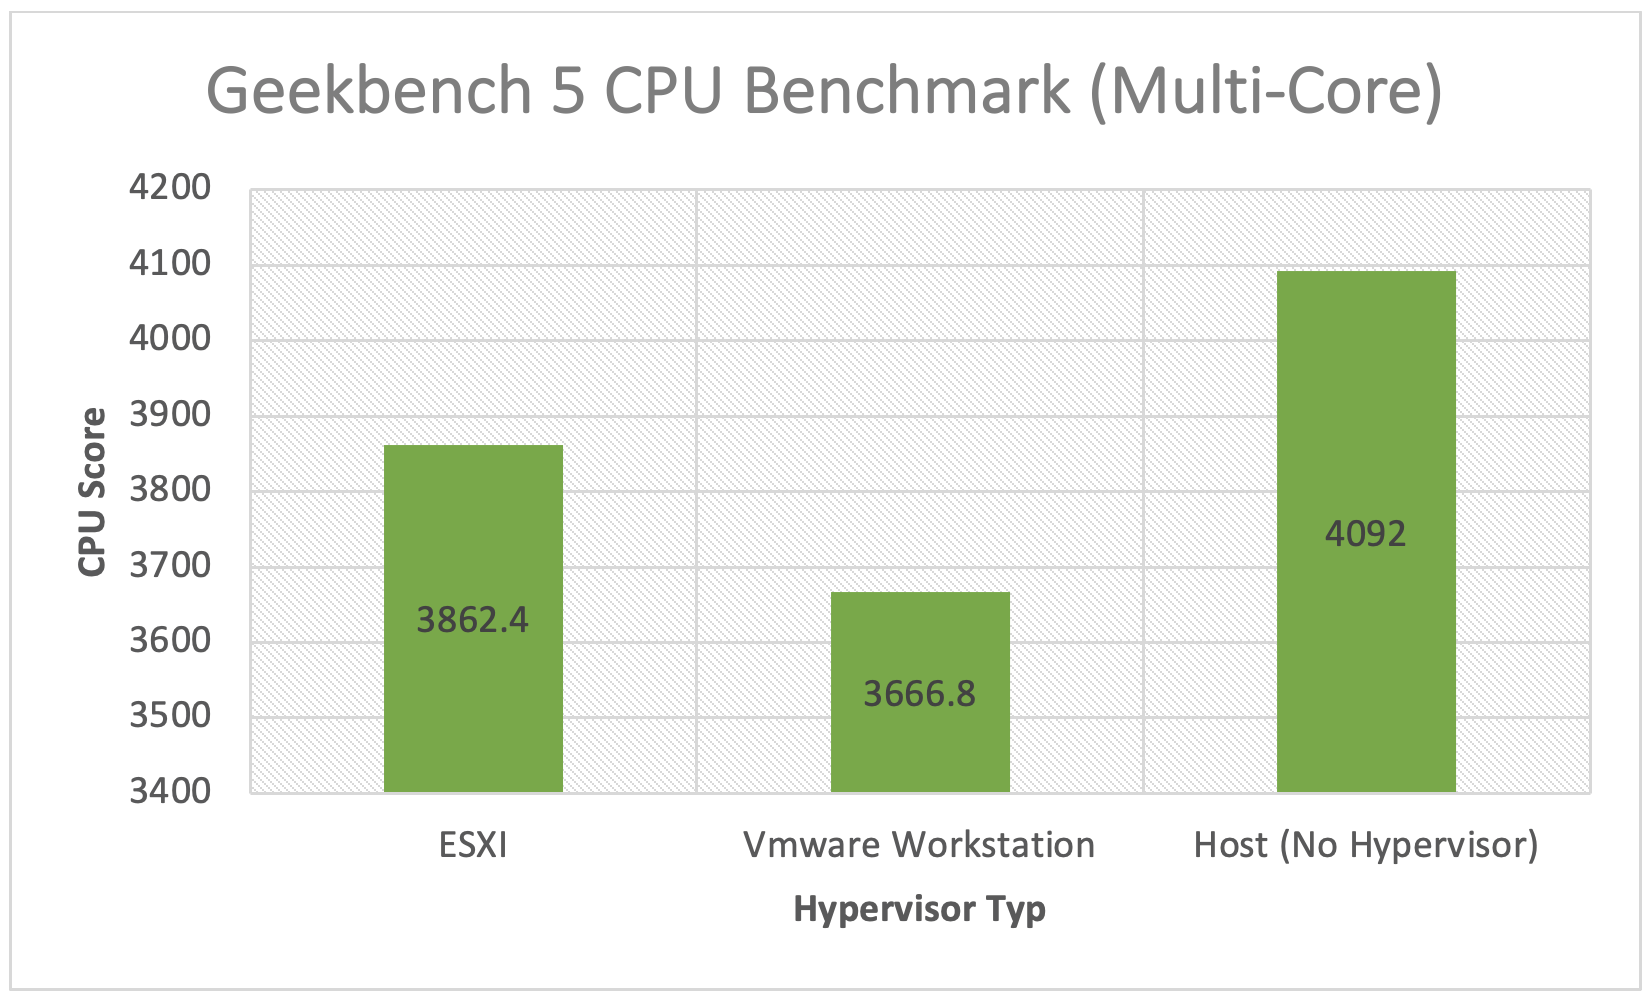
\includegraphics[keepaspectratio,width=8.5cm,height=0.75\textheight]{multicore.png}
	\caption{Multicore Benchmark}
	\label{architecture}
\end{figure}

Wie erwartet sind bei der Multicore Messung im Vergleich zum Single Core Benchmark wesentlich höhere Ergebnisse sichtbar was auf den Einsatz von insgesamt 8 Kernen (4 Kerne + 4 Threads) zurückzuführen ist. Der Typ 1 Hypvervisor erreichte in diesem Benchmark eine Punktezahl von 3862,4 Punkten und übertrifft wie erwartet die 3666,8 Punkte des VMWare Workstation Typ 1 Hypervisors. Der Unterschied zwischen Typ 1 und Typ 2 beträgt 195,6 Punkte (5,33\%) und ist somit ist der Unterschied nur marginal größer als bei der Single Core Messung (3,29\%). Wie auch beim Single Core Performance Benchmark ist auch hier der Unterschied zum Hostsystem deutlich sichtbar. Hier beträgt der Unterschied zwischen Typ 1 ESXI Hypervisor und Host 229,6 Punkte (5,94\%). Der Unterschied zwischen Typ 2 VMWare Workstation Hypervisor und Host beträgt 425,2 Punkte (11,59\%) und fällt wie erwartet höher aus. Im Vergleich zum Single Core Benchmark fällt hier jedoch der Unterschied prozentual gesehen geringer aus.

\subsection{Interpretation}
In beiden Testszenarien zeigt sich, dass das der Typ 1 Hypervisor im Vergleich zu einem Typ 2 Hypervisor eine höhere CPU-Leistung erzielen kann. Zu beginn der Arbeit wurde definiert, dass eine Leistungssteigerung von $>$10\% einen signifikanten Unterschied bedeutet. Durchschnittlich erzielt der Typ 1 Hypervisor im Vergleich zum Typ 2 Hypervisor eine 4,31% höhere Leistung (Multicore & Singlecore) und somit wird dies als nicht signifikante Leistungssteigerung betrachtet. Beachtlich war hingegen, dass im Vergleich zum Host System beide Hypervisor Typen einen erheblichen Leistungseinbruch verzeichnen müssen.

\section{Messung der Boot-Zeit}
\label{Messung der CPU Performance}
Für die Messung der Bootzeiten der VMs wurden auf beiden PCs eine Windows 10 VM mit identen Spezifikationen konfiguriert. Ursprünglich sollte dafür der Windows Log mit der ID 100 im Ereignisprotokoll als Messinstrument verwendet werden. Dieses Ereignis wird von Windows 10 standardmäßig bei jedem Bootvorgang geloggt und beinhaltet unter anderem die Bootzeit in Millisekunde. [6] Allerdings, stellte sich heraus, dass dieses Ereignis in virtuellen Umgebungen nicht erfasst werden kann. Somit wurde die Boot-Zeit durch das Filmen des Bildschirms erfasst, welches es ermöglicht den Start- und End-Frame des Bootvorganges genau festzulegen und somit auf die vergangene Zeit rückzuschließen. Für das Messergebnis wurden zwei Messungen auf den beiden PCs festgehalten und der Mittelwert berechnet.
Das Ergebnis der Bootzeitmessung ist in Abbildung 2 zu sehen. Das Booten der Windows VM auf dem Typ 2 Workstation Hypervisor dauerte etwa 70\% länger als auf dem Typ 1 Hypervisor. Ein signifikanter Unterschied, welchen wir als größer 10\% definiert haben, ist somit gegeben. Zurückzuführen ist der Unterschied auf einen geringeren Overhead von Typ 1 Hypervisoren, im Vergleich zu Typ 2 Hypervisoren, welche ein zusätzliches Hostbetriebssystem betreiben müssen. Die Abweichung zwischen den beiden Messungen war bei dem Typ 2 Hypervisor ebenfalls größer. Die erste Typ 2 Messung lag bei 18,3 Sekunden und die zweite bei 17 Sekunden. Die Typ 1 Messungen kamen bei beiden Bootvorgängen auf genau 10,4 Sekunden.

\begin{figure}[!h]
	\centering
	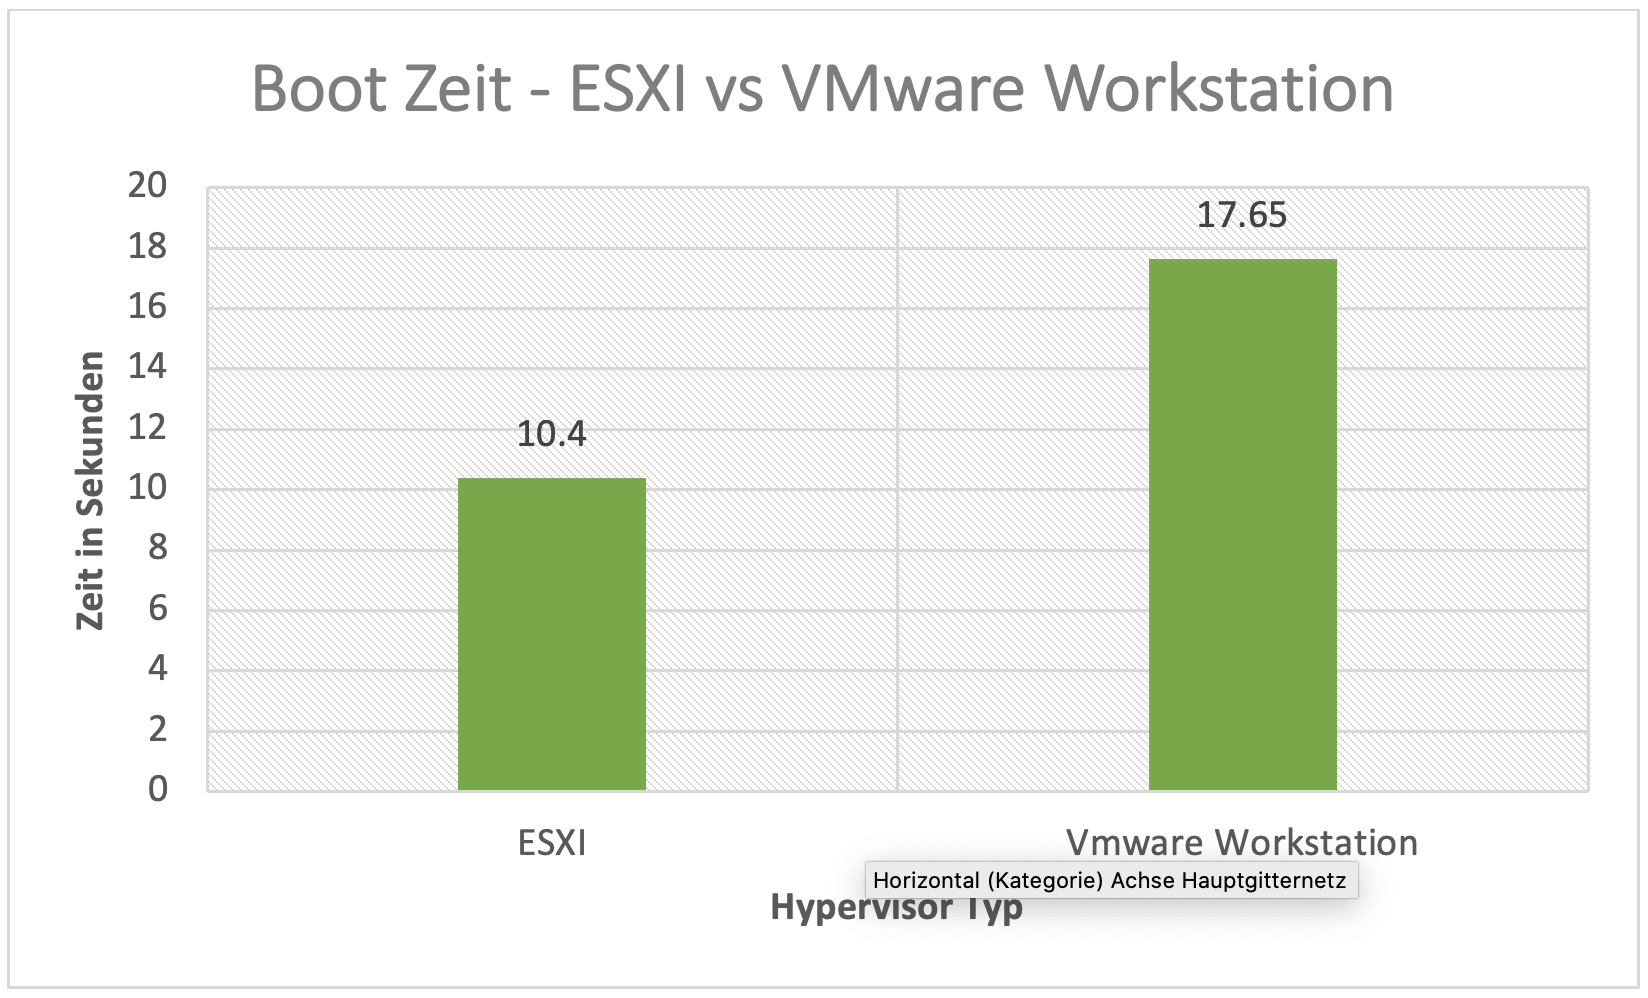
\includegraphics[keepaspectratio,width=8.5cm,height=0.75\textheight]{bootzeit.png}
	\caption{Boot Zeit Typ1 vs Typ2}
	\label{architecture}
\end{figure}

\section{Fazit}
\label{Fazit}
Lorem ipsum dolor sit amet, consetetur sadipscing elitr, sed diam nonumy eirmod tempor invidunt ut labore et dolore magna aliquyam erat, sed diam voluptua. At vero eos et accusam et justo duo dolores et ea rebum. Stet clita kasd gubergren, no sea takimata sanctus est Lorem ipsum dolor sit amet. Lorem ipsum dolor sit amet, consetetur sadipscing elitr, sed diam nonumy eirmod tempor invidunt ut labore et dolore magna aliquyam erat, sed diam voluptua. At vero eos et accusam et justo duo dolores et ea rebum. Stet clita kasd gubergren, no sea takimata sanctus est Lorem ipsum dolor sit amet. Lorem ipsum dolor sit amet, consetetur sadipscing elitr, sed diam nonumy eirmod tempor invidunt ut labore et dolore magna aliquyam erat, sed diam voluptua. At vero eos et accusam et justo duo dolores et ea rebum. Stet clita kasd gubergren, no sea takimata sanctus est Lorem ipsum dolor sit amet. Lorem ipsum dolor sit amet, consetetur sadipscing elitr, sed diam nonumy eirmod tempor invidunt ut labore et dolore magna aliquyam erat, sed diam voluptua. At vero eos et accusam et justo duo dolores et ea rebum. Stet clita kasd gubergren, no sea takimata sanctus est Lorem ipsum dolor sit amet.Lorem ipsum dolor sit amet, consetetur sadipscing elitr, sed diam nonumy eirmod tempor invidunt ut labore et dolore magna aliquyam erat, sed diam voluptua. At vero eos et accusam et justo duo dolores et ea rebum. Stet clita kasd gubergren, no sea takimata sanctus est Lorem ipsum dolor sit amet. Lorem ipsum dolor sit amet, consetetur sadipscing elitr, sed diam nonumy eirmod tempor invidunt ut labore et dolore magna aliquyam erat, sed diam voluptua. At vero eos et accusam et justo duo dolores et ea rebum. Stet clita kasd gubergren, no sea takimata sanctus est Lorem ipsum dolor sit amet. Lorem ipsum dolor sit amet, consetetur sadipscing elitr, sed diam nonumy eirmod tempor invidunt ut labore et dolore magna aliquyam erat, sed diam voluptua. At vero eos et accusam et justo duo dolores et ea rebum. Stet clita kasd gubergren, no sea takimata sanctus est Lorem ipsum dolor sit amet. Lorem ipsum dolor sit amet, consetetur sadipscing elitr, sed diam nonumy eirmod tempor invidunt ut labore et dolore magna aliquyam erat, sed diam voluptua. At vero eos et accusam et justo duo dolores et ea rebum. Stet clita kasd gubergren, no sea takimata sanctus est Lorem ipsum dolor sit amet.

\bibliographystyle{IEEEtran}
\bibliography{IEEEabrv,SEAAnew}


\end{document}
